\documentclass[11pt,a4paper]{article}
\usepackage{import}
\subimport{../../shared/}{preamble.tex}
\addbibresource{bibliography/references.bib}
\title{Reflection Projection for Validation of Experimental dq Flux Maps}
\author{}
\date{7 October 2026}
\newcommand{\PaperAbstract}{Which parts of a measured dq flux map can reflection symmetry identify and remove? Even/odd decomposition defines complementary residual channels and a unique closest symmetric pair under equal weighting. This is a projection in a declared model class, not identification of a physical fault. A portable PSM operating-point dataset is evaluated at measured current coordinates using support-limited mirror interpolation. The removed flux and the raw map remain separate outputs. Interpolation, state mismatch and genuine machine asymmetry limit physical interpretation; a constructed zero residual provides no independent calibration evidence.}
\newif\ifshowglossary\showglossarytrue
\newif\ifshowbibliography\showbibliographytrue


\begin{document}
\maketitle
\begin{abstract}
\PaperAbstract
\end{abstract}
\tableofcontents

\section{Question and contribution}
If reversing q excitation leaves the effective machine unchanged, direct-axis
flux should retain its value and quadrature-axis flux should reverse sign.
This provides a reference relationship without knowing either inductance.
The research question is which flux components this relationship detects,
and what correction can be justified from reflection alone.

Construction symmetries in energy-based motor models explain the physical
origin of reflection \cite{jebai2014}; nonlinear flux models distinguish
parity from reciprocal differential coupling \cite{sun2020}. Here we isolate
the projection implied by parity, rather than derive another magnetic model.
The contribution is an explicit closest-pair operator, an evidence boundary
for its removed component, and a measured-coordinate demonstration on a
portable PSM fixture. General causal error separation belongs to the companion
identifiability study \cite{companion-diagnostics}.
The algebra applies wherever the declared reflection and matched state hold;
experimental interpretation additionally depends on sampling and coordinates.

\section{Steady-state flux reconstruction}
Begin with the two voltage balances
\begin{align}
 \ud&=\Rs\id-\omegae\psiq, &
 \uq&=\Rs\iq+\omegae\psid.\label{eq:voltage}
\end{align}
They apply when the rotor-frame flux derivative vanishes, the represented
voltage is the terminal fundamental voltage, and the lumped resistive model
is adequate. Set
\begin{equation}
 \voltage=\begin{bmatrix}\ud\\\uq\end{bmatrix},\quad
 \current=\begin{bmatrix}\id\\\iq\end{bmatrix},\quad
 \flux=\begin{bmatrix}\psid\\\psiq\end{bmatrix},\quad
 \rotationgenerator=\begin{bmatrix}0&-1\\1&0\end{bmatrix}.
\end{equation}
Then $\rotationgenerator\flux=[-\psiq,\psid]\trans$ rotates a vector counterclockwise
through $90^\circ$, and \cref{eq:voltage} becomes
\begin{equation}
 \voltage=\Rs\current+\omegae\rotationgenerator\flux.\label{eq:vector-voltage}
\end{equation}
Subtracting the resistive drop isolates rotational EMF. Rotating it back
undoes its quadrature orientation. Since $\rotationgenerator^2=-\matr I$, for
$\omegae\ne0$ this gives
\begin{equation}
 \boxed{\flux^{\rm rec}=-\frac{1}{\omegae}\rotationgenerator
 (\voltage-\Rs\current).}\label{eq:reconstruction}
\end{equation}
Equivalently,
\begin{equation}
 \psid^{\rm rec}=\frac{\uq-\Rs\iq}{\omegae},\qquad
 \psiq^{\rm rec}=\frac{\Rs\id-\ud}{\omegae}.
\end{equation}
This operation reveals flux from the voltage balance but hides the origin of
the subtracted voltage. Any error in voltage or resistive drop is divided by
speed. At zero speed the stationary equation contains no flux information;
near zero speed the inversion amplifies noise.

Mechanical speed $n$ in revolutions per minute and pole-pair number $p$ give
\begin{equation}
 \omegae=2\pi p\frac{n}{60}.\label{eq:rpm-conversion}
\end{equation}
Requested speed labels the experimental slices below. The flux inversion
uses the mean recorded electrical angular speed of each operating point,
rather than substituting its requested breakpoint in this conversion.
Residual speed variation and upstream voltage processing remain uncertainty
sources.

No reflection symmetry follows from this inversion. Indeed, any chosen
flux-current function, symmetric or otherwise, can be inserted in
\cref{eq:vector-voltage} to produce corresponding voltages. Structural
symmetry must come from the machine, not from solving its voltage equation.
The alternative componentwise derivation gives the same signs: $u_q-R_si_q$
contains $+\omega_e\psi_d$, whereas $u_d-R_si_d$ contains
$-\omega_e\psi_q$.

\section{The physical assumption behind the reflection}
\label{sec:symmetry}
Use a rotor-aligned fundamental dq frame at fixed magnetic and thermal state.
The effective geometry, excitation and material response must be invariant
under reversing q excitation while retaining d excitation. Harmonics require
consistent averaging; history-dependent or irreversible state changes are
excluded. A machine-type label alone does not establish this assumption.

One sufficient storage description is an even normalized co-energy,
\begin{equation}
 \coenergy(i_d,i_q)=\coenergy(i_d,-i_q),\qquad
 \flux=\nabla_{\current}\coenergy.\label{eq:energy-parity}
\end{equation}
For one amplitude-invariant three-phase system this potential is physical
co-energy divided by $3/2$. Differentiation in d retains sign; differentiation
in q contributes the sign of the reflected argument. Therefore
\begin{equation}
 \psid(i_d,i_q)=\psid(i_d,-i_q),\qquad
 \psiq(i_d,i_q)=-\psiq(i_d,-i_q).\label{eq:flux-parity}
\end{equation}
A d-axis PM bias and nonlinear cross-saturation are compatible with these
equalities. The projection below needs the equalities themselves, not a fitted
potential. For example, $\psi_d=1+i_q^2$, $\psi_q=i_q$ has the required parity
but unequal mixed derivatives. Reflection and integrability answer different
questions; the latter is examined separately \cite{companion-coenergy}.

\section{Even and odd channels as diagnostic residuals}
We want to remove the legitimate symmetric magnetic structure while retaining
components that the model forbids. Compare points at equal $i_d$, temperature,
and signed speed, with opposite equal-magnitude $i_q$. Define
\begin{equation}
 \evenq[f](i_d,i_q)=\frac{f(i_d,i_q)+f(i_d,-i_q)}{2},\qquad
 \oddq[f](i_d,i_q)=\frac{f(i_d,i_q)-f(i_d,-i_q)}{2}.
 \label{eq:parity-operators}
\end{equation}
Addition retains the unchanged part; subtraction retains the reversing part.
These are complementary projections: $f=\evenq[f]+\oddq[f]$,
$\evenq^2=\evenq$, $\oddq^2=\oddq$, and $\evenq\oddq=0$. Pairing therefore discards the
allowed component in each diagnostic channel, not saturation as such.
\begin{figure}[tb]
\centering
\begin{tikzpicture}
\begin{axis}[diagnostic axis,title={Reflect the same curve},ylabel={$f(y)$},
 xmin=-1,xmax=1,ymin=.5,ymax=1.6]
 \addplot[reference quantity,strong line,domain=-1:1]{1+.2*x^2+.3*x};
 \addlegendentry{$f(y)$}
 \addplot[estimated quantity,alternative pattern,standard line,domain=-1:1]{1+.2*x^2-.3*x};
 \addlegendentry{$f(-y)$}
\end{axis}
\begin{axis}[diagnostic axis,at={(.5\textwidth,0)},anchor=south west,
 title={Average and half-difference},ylabel={Component},xmin=-1,xmax=1,ymin=-.4,ymax=1.4]
 \addplot[derived quantity,strong line,domain=-1:1]{1+.2*x^2};
 \addlegendentry{$\evenq[f]$}
 \addplot[torque quantity,standard line,domain=-1:1]{.3*x};
 \addlegendentry{$\oddq[f]$}
\end{axis}
\end{tikzpicture}
\caption{Reflection separates an illustrative curve
$f(y)=1+0.2y^2+0.3y$ into its allowed even part and its odd tilt.
The same projections applied to d and q flux select opposite diagnostic
channels. The schematic curve is not a second machine model.}
\label{fig:decomposition}
\end{figure}


For a correctly aligned ideal map, $\oddq[\psid]=0$ and $\evenq[\psiq]=0$.
Define measured residuals at the observed numerical labels by
\begin{equation}
 \boxed{r_d=\oddq[\hat\psid],\qquad r_q=\evenq[\hat\psiq].}
 \label{eq:residuals}
\end{equation}
For the independent positive-q representative $a>0$, this means explicitly
\begin{equation}
 r_d=\frac{\hat\psi_d(i_d,+a)-\hat\psi_d(i_d,-a)}{2},\qquad
 r_q=\frac{\hat\psi_q(i_d,+a)+\hat\psi_q(i_d,-a)}{2}.
\end{equation}

\subsection{Symmetry projection as a correction operator}
The same even/odd decomposition defines the closest parity-admissible pairwise map under equal weighting:
\begin{equation}
 \boxed{\psi_d^{\rm sym}=\evenq[\hat\psi_d],\qquad
        \psi_q^{\rm sym}=\oddq[\hat\psi_q].}
 \label{eq:symmetry-projection}
\end{equation}
The removed component is exactly
\begin{equation}
 \hat\flux-\flux^{\rm sym}=\begin{bmatrix}r_d\\r_q\end{bmatrix}
\end{equation}
on mirrored support. Algebraically this is an idempotent projection onto the declared parity subspace. Geometrically it folds the two measured branches onto the reflection-compatible component. Physically it is a correction only if the forbidden component is known to be nonmagnetic or otherwise inadmissible for the intended model.

A smaller symmetry residual after projection is therefore guaranteed by construction and cannot by itself validate a sensor correction, winding resistance, or rotor-angle estimate. The raw field, projected field, and removed residual must remain available separately.

\paragraph{What pairing hides.}
An allowed-parity flux error can be large and yet yield zero residuals.
A nonzero residual indicates incompatibility with the specified symmetry,
not unique proof of resistance or angle error. Interpolation mismatch,
temperature mismatch, or real machine asymmetry can enter the same channels.
Use one independent representative per pair, conventionally $i_q>0$; keeping
both representatives doubles the same information and their correlated noise.


\subsection{Why the closest pair is an average}
For two observed d values $d_+$ and $d_-$, the admissible pair is $(d,d)$.
Minimizing $(d-d_+)^2+(d-d_-)^2$ gives $d=(d_++d_-)/2$.
For q values the admissible pair is $(q,-q)$ and minimizing
$(q-q_+)^2+(-q-q_-)^2$ gives $q=(q_+-q_-)/2$.
These two one-dimensional minimizations prove the minimum-distance claim.
With unequal independent precisions $w_+,w_-$, replace the averages by
$(w_+d_++w_-d_-)/(w_++w_-)$ and
$(w_+q_+-w_-q_-)/(w_++w_-)$. Correlated uncertainty requires its full metric.
Equal weighting is a declared mathematical choice, not an inferred sensor
covariance. A normalized thought experiment $(d_+,d_-)=(3,1)$ projects to
$(2,2)$ and removes $(1,-1)$; the operator cannot tell why the difference arose.

\section{A portable measured-coordinate experiment}
The fixture \texttt{psm\_temperature\_2500} contains 680 operating points,
340 each at rotor-temperature references 30 and 70 $^\circ$C, at a requested
2500 rpm. The stored machine code is PSM and the phase selector is three-phase.
The nominal 1500-rpm variant changes six speed-related signals while retaining
all current and torque values; it is excluded as an independent experiment.

Each operating point groups logger records by requested speed, excitation,
temperature reference and measurement counter. Measured mean currents and
voltages, medians, sample deviations and counts are retained. Flux is the
stationary inversion of group means using recorded mean electrical speed and
the recorded resistance. No residual-based deletion or extra settling window
is introduced. The acquisition timing does not justify treating three stored
records as three independent calibrated repetitions.

Within each temperature slice, construct a vector-valued linear Delaunay
interpolant on measured currents. For positive q representatives above
10\% of the slice maximum $|i_q|$, evaluate its mirror at $(i_d,-i_q)$.
Keep only mirrors inside the convex hull. This addresses numerical current
matching explicitly, but introduces correlated interpolation error.
Projection is applied to the two evaluated values; we do not claim that a new
interpolant through projected vertices would automatically retain exact parity.
The raw field and removed component stay available.

\section{Measured forbidden components}
\begin{table}[htbp]\centering
\begin{tabular}{rrrrr}
\toprule
Reference / $^\circ$C & Candidates & Supported & $r_d$ RMS & $r_q$ RMS\\
\midrule
30 & 158 & 142 & 2.873 & 2.184 \\
70 & 158 & 144 & 2.477 & 2.127 \\
\bottomrule
\end{tabular}

\caption{Mirror-interpolation demonstration. Residual RMS is in mWb; support
counts describe positive-q representatives, not independent sensor trials.}
\end{table}
The observed forbidden components are on the scale of a few mWb. Their thermal
reference dependence is descriptive: a rotor reference does not establish
winding equilibrium or identify an ohmic cause. Some mirror arguments lie
outside the measured hull and are excluded instead of extrapolated.
\begin{figure}[htbp]\centering
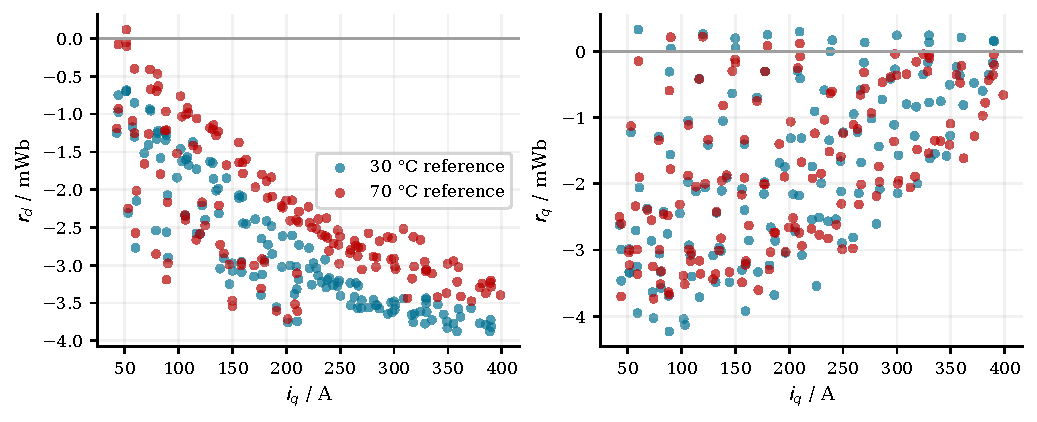
\includegraphics[width=\textwidth]{figures/real_projection.pdf}
\caption{Raw forbidden d-odd and q-even components on supported measured-current
mirrors. Separate thermal references are shown with the common visual palette.}
\label{fig:real-projection}\end{figure}
At each retained pair the projected values satisfy parity to roundoff.
That is a check of the operator, not experimental proof of a corrected machine.
An allowed-parity perturbation survives unchanged, however large it is.

\section{When projection is a physical correction}
Projection gives a unique representative in the selected parity class under
its metric. To interpret the removed component as an error one additionally
needs a qualified reflection model, matched magnetic state, aligned axes,
and an uncertainty budget that includes interpolation. Genuine construction
asymmetry or loss-state differences may be removed by the same operator.
Symmetry cannot distinguish those contributions from sensor error.

Independent calibration can justify a physical correction; symmetry alone
justifies a model projection and residual. Resistance-equivalent normalization
and geometric error fingerprints are conditional hypotheses in the companion
identifiability study \cite{companion-diagnostics}, not additional observations.

For an explicit sign regression, the generated synthetic check injects
$\varepsilon_R=\hat R_s-R_s=\SI{0.02}{\ohm}$ at
$\omega_e=\SI{1000}{\per\second}$. It reproduces
$r_d=-\varepsilon_R i_q/\omega_e$ and
$r_q=+\varepsilon_R i_d/\omega_e$ to $3.4\times10^{-21}$ Wb. Replacing the
resistance mismatch by the current-proportional voltage error
$\vect\varepsilon_u=-\varepsilon_R\current$ produces the identical reconstructed
flux perturbation to the same tolerance. Thus the resistance-equivalent pattern
is reproducible, including its sign, but resistance itself is not identifiable
from symmetry.

\section{Limits}
The demonstration has one PSM data lineage and two thermal references, not a
calibrated multi-machine validation. A P1 interpolant supplies no statistical
bound on mirror error. Repeated records may share filtering and acquisition
history. No independent true-flux field is available. Reflection says nothing
about integrability, radial flux accuracy, or errors lying in the allowed
subspace. The portable EESM and ASM fixtures support future controlled studies;
their extra state dependence prevents automatic transfer of the PSM assumption.

\section{Conclusion}
Reflection separates a map into allowed and forbidden components and gives a
closest symmetric pair under a declared metric. The measured-coordinate
demonstration exposes finite forbidden components without pretending to identify
their origin. Its scientifically justified outputs are the raw map, projected
representative, removed component and support limitations together.


\ifshowglossary
  \glsadd{pmsm}\glsadd{dq}
  \glsadd{sym:id}\glsadd{sym:iq}\glsadd{sym:rs}\glsadd{sym:omega}
  \glsadd{sym:er}\glsadd{sym:rpm}
  \printnoidxglossary[type=\acronymtype,title={Acronyms}]
  \printnoidxglossary[type=symbols,title={Symbols}]
\fi
\ifshowbibliography
  \printbibliography
\fi
\end{document}
